% Szglab4
% ===========================================================================
%
\chapter{Analízis modell kidolgozása 1}

\thispagestyle{fancy}

\section{Objektum katalógus}

\subsection{Command}
\begin{tabularx}{\linewidth}{| l | X |}
\hline
\textbf{Név} & \textbf{Leírás} \tabularnewline
\hline\hline
\endhead
ChangeDirectionQuery & Egy robottól irányváltoztatást kérő parancs. Elő tudja állítani a megfelelő \textbf{ChangeDirectionTransmit} parancsot. \tabularnewline\hline

ChangeDirectionTransmit & Az az irányváltoztató parancs, amit egy cella módosítani tud a rajta található buffokkal. Elő tudja állítani a megfelelő \textbf{ChangeDirectionExecute} parancsot. \tabularnewline\hline 

ChangeDirectionExecute & Az ugrást a \textbf{Roboton} ténylegesen végrehajtó parancs. \tabularnewline\hline

ChangeSpeedQuery & Egy robottól sebességváltoztatást kérő parancs. Elő tudja állítani a megfelelő \textbf{ChangeSpeedTransmit} parancsot. \tabularnewline\hline

ChangeSpeedTransmit & Az a sebességváltoztató parancs, amit egy cella módosítani tud a rajta található buffokkal. Elő tudja állítani a megfelelő \textbf{ChangeSpeedExecute} parancsot. \tabularnewline\hline

ChangeSpeedExecute & A sebességváltoztatást a \textbf{Roboton} ténylegesen végrehajtó parancs. \tabularnewline\hline

JumpQuery & Egy robottól ugrás kezdeményezését kérő parancs. Lekérdezi és tárolja a robot aktuális sebességét. Elő tudja állítani a megfelelő \textbf{JumpTransmit} parancsot.  \tabularnewline\hline

JumpTransmit & Az az ugróparancs, amit egy cella módosítani tud a rajta található buffokkal. Lekérdezi a cellától az ugrás kezdetét és célját, és tárolja ezeket. Elő tudja állítani a megfelelő \textbf{JumpExecute} parancsot. \tabularnewline\hline 

JumpExecute & Az ugrást a \textbf{Roboton}, a kezdő és cél cellán ténylegesen végrehajtó parancs. \tabularnewline\hline

KillExecute & Egy \textbf{Robotot} a játékból kiiktatni képes parancs. \tabularnewline\hline

TimoutExecute & Egy \textbf{Robotnak} jelzi, hogy elfogyott a rá kijelölt teljes időtartam. \tabularnewline\hline

UseOilQuery & Egy \textbf{Robotot} arra utasít, hogy helyezzen egy \textbf{Oil} buffot arra a mezőre, amelyen áll. Lekérdezi, hogy a robotnak van-e elérhető \textbf{Oil} készlete, és ezt tárolja. Elő tudja állítani a megfelelő \textbf{UseOilExecute} parancsot. \tabularnewline\hline

UseOilExecute & Egy \textbf{Oil} buffot helyez el a cellán. \tabularnewline\hline

UseStickyQuery & Egy \textbf{Robotot} arra utasít, hogy helyezzen egy \textbf{Sticky} buffot arra a mezőre, amelyen áll. Lekérdezi, hogy a robotnak van-e elérhető \textbf{Sticky} készlete, és ezt tárolja. Elő tudja állítani a megfelelő \textbf{UseStickyExecute} parancsot. \tabularnewline\hline

UseStickyExecute & Egy \textbf{Sticky} buffot helyez el a cellán. \tabularnewline\hline
\end{tabularx}

\subsection{Direction}
Tárolja egy \textbf{Robot} lehetséges mozgási irányait, és egyben a megfelelő \textbf{Cellek} lehetséges szomszédossági viszonyait.

\subsection{EmptyFieldCell}
Az \textbf{EmptyFieldCell} osztály példányai a pálya azon részeit tárolja, amelyre lépve a \textbf{Robotok} kiesnek a játékból. Az ő felelőssége a robotnak elküldeni azt a parancsot, ami ezt a hatást előidézi (\textbf{KillExecute}).
Tárolja a rajta álló robotot, illetve referenciákat a szomszédos mezőkre, amiket a megfelelő \textbf{Direction} megadásával érhetünk el. Tartalmazza ezen felül a céltól való távolságot, amelyet a nyertes meghatározására használhatunk. Az ő felelőssége annak a cellának a megkeresése, amelyre egy \textbf{Robot} ugorhat. A cellán átmenő parancsokat módosíthatja a rajta található buffokkal.

\subsection{FieldCell}
Ezen osztály példányai alkotják a pálya legnagyobb részét: minden olyan cella, amely nem a célvonal része, illetve nem a pálya szélét alkotja ilyen típusú. A \textbf{FieldCell} példányok fontos feldata, hogy a rálépő \textbf{Robotokon} érvényesítse a cellán lévő buffokat. Ezen felül a \textbf{Robotoknak} érkező parancsok egy része keresztülhalad ezeken a mezőkön, ahol a rajta található buffok ezeket a parancsokat módosíthatják. A \textbf{FieldCell} ezután a módosított parancsot
továbbítja a rajta álló \textbf{Robot} felé.
Tárolja a rajta álló robotot, illetve referenciákat a szomszédos mezőkre, amiket a megfelelő \textbf{Direction} megadásával érhetünk el. Tartalmazza ezen felül a céltól való távolságot, amelyet a nyertes meghatározására használhatunk. Az ő felelőssége annak a cellának a megkeresése, amelyre egy \textbf{Robot} ugorhat. A cellán átmenő parancsokat módosíthatja a rajta található buffokkal.

\subsection{FinishLineFieldCell}
A \textbf{FinishLineFieldCell} osztály példányainak felelősségei megegyeznek a \textbf{FieldCell} osztály példányainak felelősségeivel, azzal a különbséggel, hogy ezek a cellák jelzik egy körnek a végét.

\subsection{Inventory}
Buffok tárolására alkalmas, nyílvántartja a benne található buffok számát, és csak akkor engedi azokat használni, ha legalább egyet tartalmaz.

\subsection{Oil}
Egy olyan buff, aminek hatására a \textbf{Fieldre} lépő \textbf{Robotok} sebessége megfelelződik.

\subsection{Result}
Egy parancs lefutásának eredményét tárolja.

\subsection{Robot}
A \textbf{Robot} osztály példányai egy-egy pályán mozgó robotot tárolnak. Tárolja a saját sebességét, illetve azt a cellát, amin pillanatnyilag áll. Ezen felül rendelkeznek \textbf{Inventorykkal}, amelyben \textbf{Stickyt} vagy \textbf{Oilt} tárolnak. Ezeket le tudják helyezni arra a cellára, amelyen állnak.

\subsection{Speed}
Egy \textbf{Robot} sebességét reprezentálja.

\subsection{Sticky}
Egy olyan buff, ami képes a \textbf{JumpExecute} parancs olyan módosítására, amely megakadályozza azt, hogy ez a parancs megváltoztassa egy \textbf{Robot} sebességét.


\begin{figure}[h]
\begin{center}
%\includegraphics[width=17cm]{chapters/chapter03/example.pdf}
\caption{x}
\label{fig:example1}
\end{center}
\end{figure}


\section{Osztályok leírása}

\subsection{Agent (Abstract)}
\begin{itemize}

\item Felelősség\\
A pályán lévő összes ágens közös viselkedését valósítja meg: tárolja azoknak a sebességét, azt a \textbf{Fieldet}, amelyen éppen áll. Ezen felül számon tartja azt is, hogy az \textbf{Agent} élő vagy halott állapotban van-e, illetve hogy elfogyott-e már az adott \textbf{Agentre} osztott idő.

\item Ősosztályok\\
Nincs

\item Interfészek\\
AgentElement

\item Attribútumok\\
\begin{itemize}
    \item field: Field
    \item speed: Speed
    \item isDead: bool
    \item isOutOfTime: bool
    \item currentLeft: int
\end{itemize}

\item Metódusok\\

\begin{itemize}
    \item Speed getSpeed(): visszaadja az \textbf{Agent} sebességét
    \item void setSpeed(speed: Speed): beállítja az \textbf{Agent} sebességét
    \item Field getField(): visszaadja a mezőt, ahol az \textbf{Agent} áll
    \item void setField(field: Field): beállítja, hogy melyik mezőn áll az \textbf{Agent}
    \item bool isDead(): megmondja, hogy \textbf{Agent} halott-e
    \item void kill(): megöli az \textbf{Agentet}
    \item bool isOutOfTime(): megmondja, hogy az \textbf{Agentnek} van-e még ideje lépni
    \item void timeOut(): jelzi az \textbf{Agent} felé, hogy lejárt az ideje
    \item void getLap(): megmondja, hogy hányadik körben van az \textbf{Agent}
    \item void incrementLap(): növeli a kör számlálóját
\end{itemize}

\end{itemize}

\subsection{AgentCommand (Abstract)}
\begin{itemize}

\item Felelősség\\
Az Agentre vonatkozó parancsok közös ősosztálya, az azokra jellemző közös viselkedést valósítja meg.

\item Ősosztályok\\
Nincs

\item Interfészek\\
AgentVisitor

\item Attribútumok\\
Nincs

\item Metódusok\\

\begin{itemize}
    \item FieldCommand getFieldCommand(): amennyiben a parancsláncban szükeséges egy mezőnek átadni a parancsot, ezt állítja elő.
    \item void accept(element: AgentCommandVisitor): a \textbf{AgentCommandeket} módosítani képes objektumok ezen keresztül tudják ezt megtenni
\end{itemize}

\end{itemize}

\subsection{AgentCommandVisitor (Interface)}
\begin{itemize}

\item Felelősség\\
    Ezen interfészt implementáló osztályok képessé válnak az \textbf{AgentCommand} absztrakt osztály leszármazott osztályainak megváltoztatására képes azoknak publikus interfészén keresztül.

\item Ősosztályok\\
Nincs

\item Interfészek\\
Nincs

\item Attribútumok\\
Nincs

\item Metódusok\\

\begin{itemize}
    \item void visit(element: JumpQuery): egy \textbf{JumpQuery} objektum módosítására képes annak publikus interfészén keresztül
    \item void visit(element: UseOilQuery): egy \textbf{UseOilQuery} objektum módosítására képes annak publikus interfészén keresztül
    \item void visit(element: UseStickyQuery): egy \textbf{UseStickyQuery} objektum módosítására képes annak publikus interfészén keresztül
    \item void visit(element: ChangeDirectionQuery): egy \textbf{ChangeDirectionQuery} objektum módosítására képes annak publikus interfészén keresztül
    \item void visit(element: ChangeSpeedQuery): egy \textbf{ChangeSpeedQuery} objektum módosítására képes annak publikus interfészén keresztül
    \item void visit(element: KillExecute): egy \textbf{KillExecute} objektum módosítására képes annak publikus interfészén keresztül
    \item void visit(element: TimeoutExecute): egy \textbf{TimeoutExecute} objektum módosítására képes annak publikus interfészén keresztül
    \item void visit(element: JumpExecute): egy \textbf{JumpExecute} objektum módosítására képes annak publikus interfészén keresztül
    \item void visit(element: ChangeDirectionExecute): egy \textbf{ChangeDirectionExecute} objektum módosítására képes annak publikus interfészén keresztül
    \item void visit(element: ChangeSpeedExecute): egy \textbf{ChangeSpeedExecute} objektum módosítására képes annak publikus interfészén keresztül
\end{itemize}

\end{itemize}


\subsection{AgentElement (Interface)}
\begin{itemize}

\item Felelősség\\
Ez az interfész előírja, hogy az őt implementáló osztályoknak képesnek kell lennie \textbf{AgentVisitorok} és \textbf{AgentCommandek} fogadására. 

\item Ősosztályok\\
Nincs

\item Interfészek\\
Nincs

\item Attribútumok\\
Nincs

\item Metódusok\\

\begin{itemize}
    \item void accept(visitor: AgentVisitor): ez a metódus képes az \textbf{AgentVisitor} fogadására
    \item void accept(visitor: AgentCommand): ez a metódus képes az \textbf{AgentCommand} fogadására
\end{itemize}

\end{itemize}

\subsection{AgentVisitor (Interface)}
\begin{itemize}

\item Felelősség\\
Ezen interfészt implementáló osztályok képessé válnak az \textbf{Agent} absztrakt osztály leszármazott osztályainak megváltoztatására, azoknak publikus interfészén keresztül.

\item Ősosztályok\\
Nincs

\item Interfészek\\
Nincs

\item Attribútumok\\
Nincs

\item Metódusok\\

\begin{itemize}
    \item void visit(element: Robot): egy \textbf{Robot} módosítása annak publikus interfészén keresztül
\end{itemize}

\end{itemize}

\subsection{Buff (Abstract)}
\begin{itemize}

\item Felelősség\\
    Az összes releváns Visitornak biztosít egy üres implementációt, illetve közös ősosztály biztosít a játékban található \textbf{Buffoknak}. Ezek segítségével érhető el, hogy a játékos által kiadott parancsok és az \textbf{Agentek} tetszőlegesen módosíthatók legyenek. Interface collection.

\item Ősosztályok\\
Nincs

\item Interfészek\\
FieldCommandVisitor\\
AgentCommandVisitor\\
AgentVisitor\\

\item Attribútumok\\
Nincs

\item Metódusok\\
Nincs

\end{itemize}

\subsection{Command (Abstract)}
\begin{itemize}

\item Felelősség\\
    Az összes parancs közös ősosztály, tárolja azt az állapotot, hogy az adott parancs éppen futtatható-e. A parancsok általános feladata az \textbf{Agentek} és \textbf{Fieldek} közötti kommunikáció, illetva az azokkal való interakció megvalósítása. A parancsok részletes leírása a \textit{Command (Abstract)} pont alján található táblázatban látható.

\item Ősosztályok\\
Nincs

\item Interfészek\\
Nincs

\item Attribútumok\\
    \begin{itemize}
            \item canExecute: bool
    \end{itemize}

\item Metódusok\\

\begin{itemize}
    \item bool canExecute(): igazzal tér vissza, ha a parancs végrehajtható
    \item bool setExecutable(canExecute: bool): beállítja, hogy futtatható-e a parancs
\end{itemize}

\end{itemize}

\begin{tabularx}{\linewidth}{| p{4cm} | X | p{2.5cm} | l | p{1.2cm} | p{1.2cm} |}
\hline
\textbf{Név} & \textbf{Felelősség} & \textbf{Ősosztályok} & \textbf{Interfészek} &\parbox[t]{1.2cm}{\textbf{Attribú-tumok}} & \parbox[t]{1.2cm}{\textbf{Metó-dusok}} \tabularnewline
\hline\hline
\endhead
ChangeDirectionQuery & Egy robottól irányváltoztatást kérő parancs. Elő tudja állítani a megfelelő \textbf{ChangeDirectionTransmit} parancsot. & AgentCommand, Command & AgentVisitor & - & - \tabularnewline\hline

ChangeDirectionTransmit & Az az irányváltoztató parancs, amit egy cella módosítani tud a rajta található buffokkal. Elő tudja állítani a megfelelő \textbf{ChangeDirectionExecute} parancsot. &  FieldCommand, Command & FieldVisitor & - & -\tabularnewline\hline 

ChangeDirectionExecute & Az ugrást a \textbf{Roboton} ténylegesen végrehajtó parancs. & AgentCommand, Command & AgentVisitor & - & - \tabularnewline\hline

ChangeSpeedQuery & Egy robottól sebességváltoztatást kérő parancs. Elő tudja állítani a megfelelő \textbf{ChangeSpeedTransmit} parancsot. & AgentCommand, Command & AgentVisitor & - & - \tabularnewline\hline

ChangeSpeedTransmit & Az a sebességváltoztató parancs, amit egy cella módosítani tud a rajta található buffokkal. Elő tudja állítani a megfelelő \textbf{ChangeSpeedExecute} parancsot. &  FieldCommand, Command & FieldVisitor & - & -\tabularnewline\hline

ChangeSpeedExecute & A sebességváltoztatást a \textbf{Roboton} ténylegesen végrehajtó parancs. & AgentCommand, Command & AgentVisitor & - & - \tabularnewline\hline

JumpQuery & Egy robottól ugrás kezdeményezését kérő parancs. Lekérdezi és tárolja a robot aktuális sebességét. Elő tudja állítani a megfelelő \textbf{JumpTransmit} parancsot. & AgentCommand, Command & AgentVisitor & - & - \tabularnewline\hline

JumpTransmit & Az az ugróparancs, amit egy cella módosítani tud a rajta található buffokkal. Lekérdezi a cellától az ugrás kezdetét és célját, és tárolja ezeket. Elő tudja állítani a megfelelő \textbf{JumpExecute} parancsot. &  FieldCommand, Command & FieldVisitor & - & -\tabularnewline\hline 

JumpExecute & Az ugrást a \textbf{Roboton}, a kezdő és cél cellán ténylegesen végrehajtó parancs. & AgentCommand, Command & AgentVisitor & - & - \tabularnewline\hline

KillExecute & Egy \textbf{Robotot} a játékból kiiktatni képes parancs. & AgentCommand, Command & AgentVisitor & - & - \tabularnewline\hline

TimoutExecute & Egy \textbf{Robotnak} jelzi, hogy elfogyott a rá kijelölt teljes időtartam. & AgentCommand, Command & AgentVisitor & - & - \tabularnewline\hline

UseOilQuery & Egy \textbf{Robotot} arra utasít, hogy helyezzen egy \textbf{Oil} buffot arra a mezőre, amelyen áll. Lekérdezi, hogy a robotnak van-e elérhető \textbf{Oil} készlete, és ezt tárolja. Elő tudja állítani a megfelelő \textbf{UseOilExecute} parancsot. & AgentCommand, Command & AgentVisitor & - & - \tabularnewline\hline

UseOilExecute & Egy \textbf{Oil} buffot helyez el a cellán. &  FieldCommand, Command & FieldVisitor & - & -\tabularnewline\hline

UseStickyQuery & Egy \textbf{Robotot} arra utasít, hogy helyezzen egy \textbf{Sticky} buffot arra a mezőre, amelyen áll. Lekérdezi, hogy a robotnak van-e elérhető \textbf{Sticky} készlete, és ezt tárolja. Elő tudja állítani a megfelelő \textbf{UseStickyExecute} parancsot. & AgentCommand, Command & AgentVisitor & - & - \tabularnewline\hline

UseStickyExecute & Egy \textbf{Sticky} buffot helyez el a cellán. &  FieldCommand, Command & FieldVisitor & - & -\tabularnewline\hline
\end{tabularx}

\subsection{Direction}
\begin{itemize}

\item Felelősség\\
A pályán értelmezett lehetséges irányokat jelképező enumerált típus.

\item Ősosztályok\\
Nincs

\item Interfészek\\
Nincs

\item Attribútumok\\
Nincs

\item Metódusok\\
Nincs

\end{itemize}

\subsection{Displacement}
\begin{itemize}

\item Felelősség\\
Az elmozdulást kezelő osztály, mely a kezdeti és végpont mezőket tárolja.

\item Ősosztályok\\
Nincs

\item Interfészek\\
Nincs

\item Attribútumok\\
    \begin{itemize}
            \item start: Field
            \item goal: Field
    \end{itemize}

\item Metódusok\\

\begin{itemize}
    \item Field getStart(): visszaadja a kezdeti mezőt
    \item Field getGoal(): visszaadja az érkezési mezőt
\end{itemize}

\end{itemize}

\subsection{EmptyFieldCell}
\begin{itemize}

\item Felelősség\\
Az \textbf{EmptyFieldCell} osztály példányai a pálya azon részeit tárolja, amelyre lépve a \textbf{Robotok} kiesnek a játékból. Az ő felelőssége a robotnak elküldeni azt a parancsot, ami ezt a hatást előidézi (\textbf{KillExecute}).

\item Ősosztályok\\
Field

\item Interfészek\\
FieldElement

\item Attribútumok\\
Nincs

\item Metódusok\\
Nincs

\end{itemize}

\subsection{Field (Abstract)}
\begin{itemize}

\item Felelősség\\
    A pályát alkotó mezőtípusok közös ősosztálya, biztosítja a közös funkciók megvalósítását. Tárolja a rajta álló robotot, illetve referenciákat a szomszédos mezőkre, amiket a megfelelő \textbf{Direction} megadásával érhetünk el. Tartalmazza ezen felül a céltól való távolságot, amelyet a nyertes meghatározására használhatunk. Az ő felelőssége annak a cellának a megkeresése, amelyre egy \textbf{Robot} ugorhat. 

\item Ősosztályok\\
Nincs

\item Interfészek\\
Nincs

\item Attribútumok\\
    \begin{itemize}
            \item agent: Agent
            \item distanceFromGoal: int 
            \item buffs: Buff[]
            \item neighbours: Map<Direction, Field>
    \end{itemize}

\item Metódusok\\

\begin{itemize}
    \item void addNeighbour(direction: Direction, field: Field): hozzáadja a mezőhöz a megfelelő szomszédot a megfelelő irányban.
    \item void onEnter(agent: Agent): lekezeli azt az esetet, amikor egy \textbf{Agent} a cellára lép: beállítja a megfelelő referenciákat (mind az \textbf{Agentben}, mint önmagában). Ezen felül meghívja a rálépő \textbf{Agent} \textit{accept(AgentVisitor)} metódusát az összes, a mezőn található \textbf{Buffal}. 
    \item void onExit(): lekezeli azt az esetet, amikor egy \textbf{Agent} elhagyja a mezőt
    \item int getDistanceFromGoal(): megmondja, hogy a mező hány mezőre van a céltól.
    \item void placeBuff(buff: Buff): a paraméterben megadott buffot a mezőre teszi
    \item Displacement getDisplacement(speed: Speed): kiszámolja, hogy adott sebességgel melyik másik \textbf{Fieldre} lehet ugrani.
\end{itemize}

\end{itemize}

\subsection{FieldCell}
\begin{itemize}

\item Felelősség\\
    Ezen osztály példányai alkotják a pálya legnagyobb részét: minden olyan cella, amely nem a célvonal része, illetve nem a pálya szélét alkotja ilyen típusú. A \textbf{Field} osztály által implementált tulajdonságok mellett A cellán átmenő parancsokat módosíthatja a rajta található
    \textbf{Buffokal}, majd a módosított parancsokat továbbítja a rajta álló \textbf{Agent} felé.

\item Ősosztályok\\
Field

\item Interfészek\\
(Field) - FieldElement

\item Attribútumok\\
Nincs

\item Metódusok\\
Nincs

\end{itemize}

\subsection{FieldCommand (Abstract)}
\begin{itemize}

\item Felelősség\\
    A \textbf{Fieldre} vonatkozó parancsok közös ősosztálya, az azokra jellemző közös viselkedést valósítja meg.

\item Ősosztályok\\
Nincs

\item Interfészek\\
FieldVisitor

\item Attribútumok\\
Nincs

\item Metódusok\\

\begin{itemize}
    \item AgentCommand getAgentCommand(): amennyiben a parancsláncban szükeséges egy \textbf{Agentnek} átadni a parancsot, ezt állítja elő.
    \item void accept(element: FieldCommandVisitor): a \textbf{FieldCommandeket} módosítani képes objektumok ezen keresztül tudják ezt megtenni\end{itemize}

\end{itemize}

\subsection{FieldCommandVisitor (Interface)}
\begin{itemize}

\item Felelősség\\
    Ezen interfészt implementáló osztályok képessé válnak a \textbf{FieldCommand} absztrakt osztály leszármazott osztályainak megváltoztatására képes azoknak publikus interfészén keresztül.

\item Ősosztályok\\
Nincs

\item Interfészek\\
Nincs

\item Attribútumok\\
Nincs

\item Metódusok\\

\begin{itemize}
    \item void visit(element: JumpTransmit): egy JumpTransmit objektum módosítására képes annak publikus interfészén keresztül
    \item void visit(element: UseOilExecute): egy UseOilExecute objektum módosítására képes annak publikus interfészén keresztül
    \item void visit(element: UseStickyExecute): egy UseStickyExecute objektum módosítására képes annak publikus interfészén keresztül
    \item void visit(element: ChangeDirectionTransmit): egy ChangeDirectionTransmit objektum módosítására képes annak publikus interfészén keresztül
    \item void visit(element: ChangeSpeedTransmit): egy ChangeSpeedTransmit objektum módosítására képes annak publikus interfészén keresztül
\end{itemize}

\end{itemize}

\subsection{FieldElement (Interface)}
\begin{itemize}

\item Felelősség\\
    Ez az interfész előírja, hogy az őt implementáló osztályoknak képesnek kell lennie \textbf{FieldVisitorok} és \textbf{FieldCommandek} fogadására. 

\item Ősosztályok\\
Nincs

\item Interfészek\\
Nincs

\item Attribútumok\\
Nincs

\item Metódusok\\

\begin{itemize}
    \item void accept(visitor: FieldVisitor): ez a metódus képes a \textbf{FieldVisitor} fogadására
    \item void accept(visitor: FieldCommand): ez a metódus képes a \textbf{FieldCommand} fogadására
\end{itemize}

\end{itemize}

\subsection{FinishLineFieldCell}
\begin{itemize}

\item Felelősség\\
    A célt jelző mezőtípus, a körök nyomonkövetésekor használt mező. Viselkedése egyébként megegyezik a \textbf{FieldCellével}.

\item Ősosztályok\\
Field

\item Interfészek\\
(Field) - FieldElement

\item Attribútumok\\
Nincs

\item Metódusok\\
Nincs

\end{itemize}

\subsection{FieldVisitor (Interface)}
\begin{itemize}

\item Felelősség\\
Ezen interfészt implementáló osztályok képessé válnak a Field absztrakt osztály leszármazott osztályainak módosítására, megváltoztatására, azoknak publikus interfészén keresztül.

\item Ősosztályok\\
Nincs

\item Interfészek\\
Nincs

\item Attribútumok\\
Nincs

\item Metódusok\\

\begin{itemize}
    \item void visit(element: FieldCell): egy \textbf{FieldCell} objektum módosítására képes annak publikus interfészén keresztül
    \item void visit(element: EmptyFieldCell): meglátogat egy \textbf{EmptyFieldCell} objektumot
    \item void visit(element: FinishLineFieldCell): egy \textbf{FinishLineFieldCell} objektum módosítására képes annak publikus interfészén keresztül
\end{itemize}

\end{itemize}

\subsection{Inventory<T>}
\begin{itemize}

\item Felelősség\\
    \textbf{Buffok} tárolására alkalmas tároló: számon tartja az elérhető buffok számát, így csak akkor használható, amikor nem üres.

\item Ősosztályok\\
Nincs

\item Interfészek\\
Nincs

\item Attribútumok\\
\begin{itemize}
    \item buffs: T[]
\end{itemize}

\item Metódusok\\

\begin{itemize}
    \item void addItem(item: T): hozzáad egy T típusú itemet az Inventory<T>-hez.
    \item bool useItem(): használja az Inventory<T>-ben tárolt itemet, amennyiben nem üres igazzal tér vissza, különben hamis.
\end{itemize}

\end{itemize}

\subsection{Robot}
\begin{itemize}

\item Felelősség\\
    A pályán elhelyezkedő egyik \textbf{Agent} típus. Az ősosztályban megvalósított tulajdonságokon kívül rendelkezik \textbf{Sticky} és \textbf{Oil} \textbf{Inventorykkal}, amelyeket a \textbf{Robot} tetszőlegesen használhat, ha azok nem üresek.

\item Ősosztályok\\
Agent

\item Interfészek\\
(Agent) - AgentElement

\item Attribútumok\\
\begin{itemize}
    \item stickyInventory: Inventory<Sticky>
    \item oilInventory: Inventory<Oil>
    \item buffs: Buff[]
\end{itemize}
\end{itemize}

\subsection{Speed}
\begin{itemize}

\item Felelősség\\
    A sebesség tárolására alkalmas osztály, amely egy irányt (\textbf{Direction}) és egy nagyságot tárol.

\item Ősosztályok\\
Nincs

\item Interfészek\\
Nincs

\item Attribútumok\\
\begin{itemize}
    \item direction: Direction
    \item magnitude: int

\end{itemize}

\item Metódusok\\

\begin{itemize}
    \item Direction getDirection(): a sebesség irányát adja vissza
    \item int getMagnitude(): a sebesség nagyságát adja vissza
    \item void setDirection(dir: Direction): beállítja a sebesség irányát
    \item void setMagnitude(magnitude: int): beállítja a sebesség nagyságát
\end{itemize}

\end{itemize}

\clearpage

\section{Statikus struktúra diagramok}

\begin{figure}[h]
\begin{center}
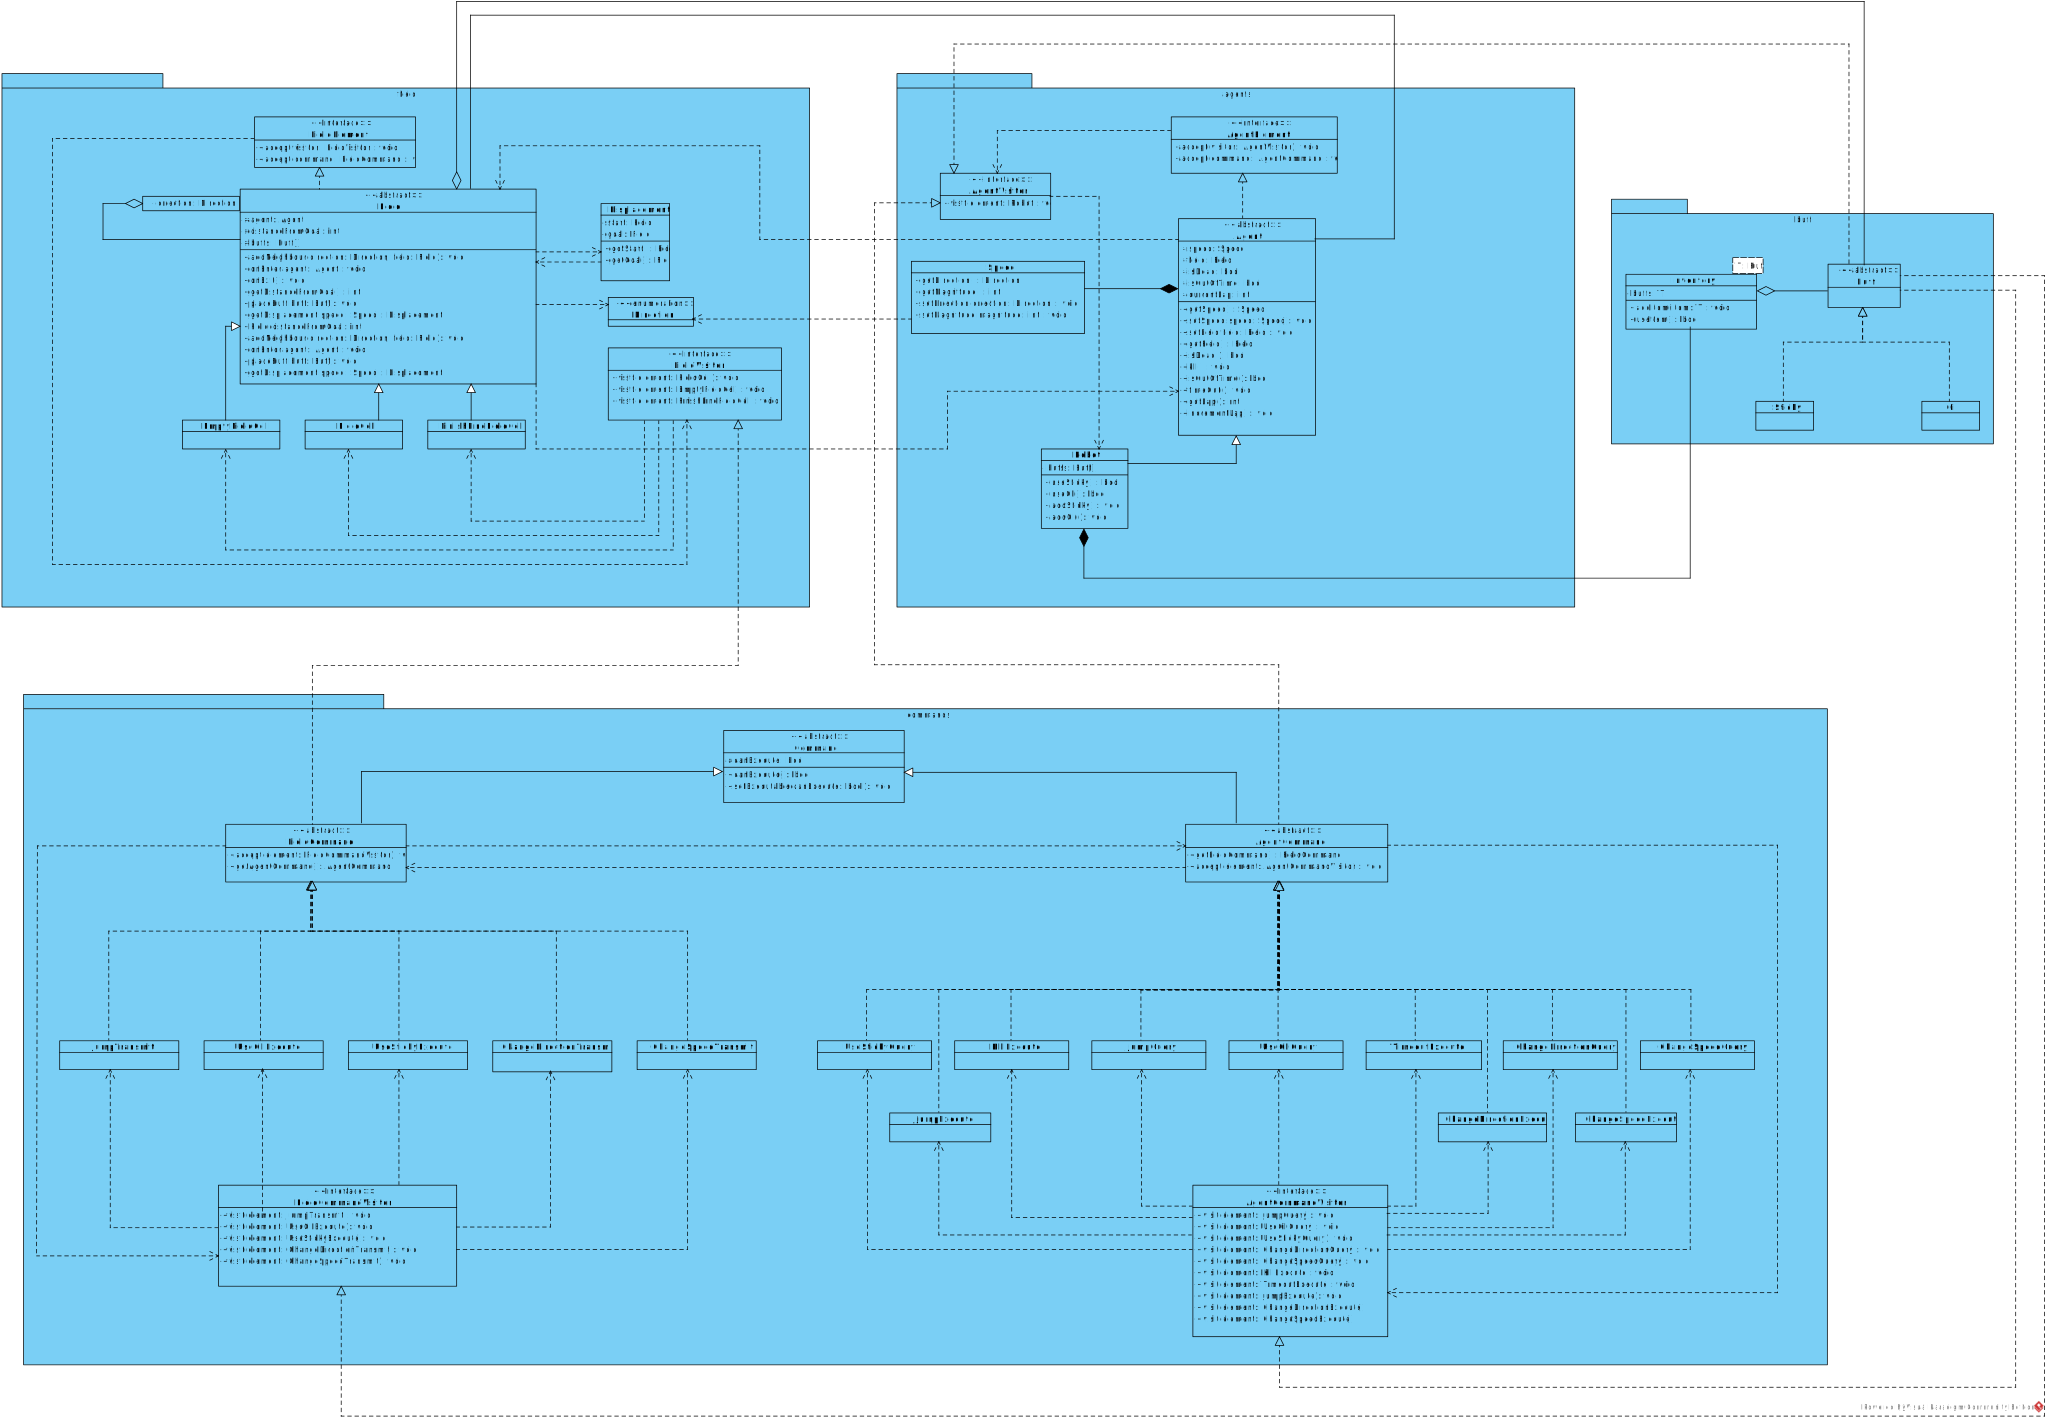
\includegraphics[width=\linewidth]{chapters/chapter03/ClassMain.pdf}
\caption{A teljes osztálydiagram}
\label{A teljes osztálydiagram}
\end{center}
\end{figure}

\begin{figure}[h]
\begin{center}
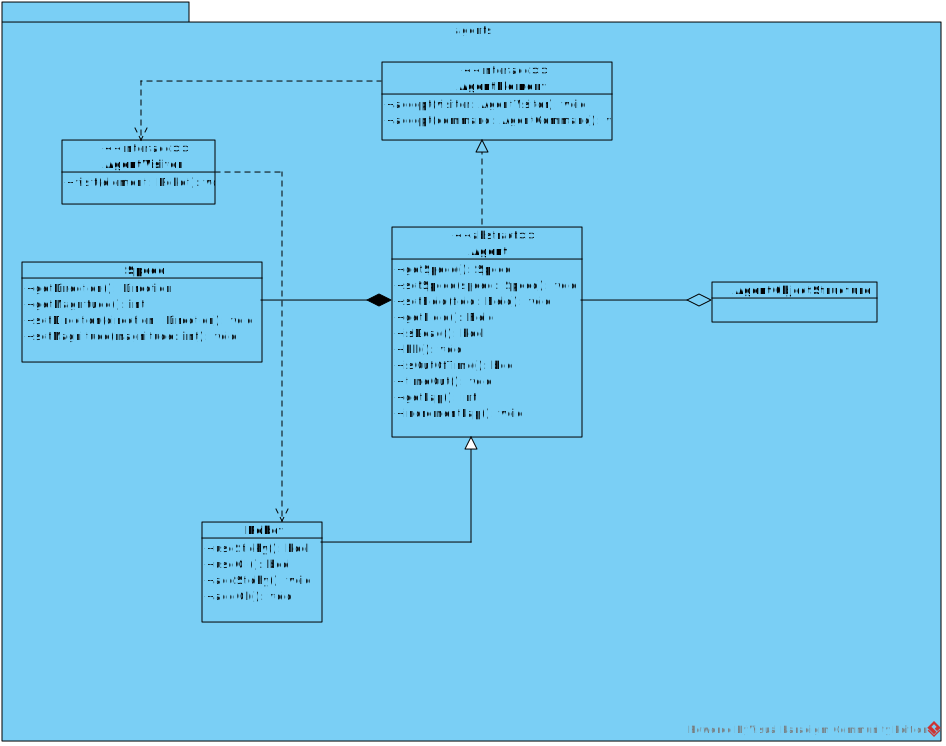
\includegraphics[width=\linewidth]{chapters/chapter03/ClassAgents.pdf}
\caption{Agents package osztálydiagram}
\label{Agents package osztálydiagram}
\end{center}
\end{figure}

\begin{figure}[h]
\begin{center}
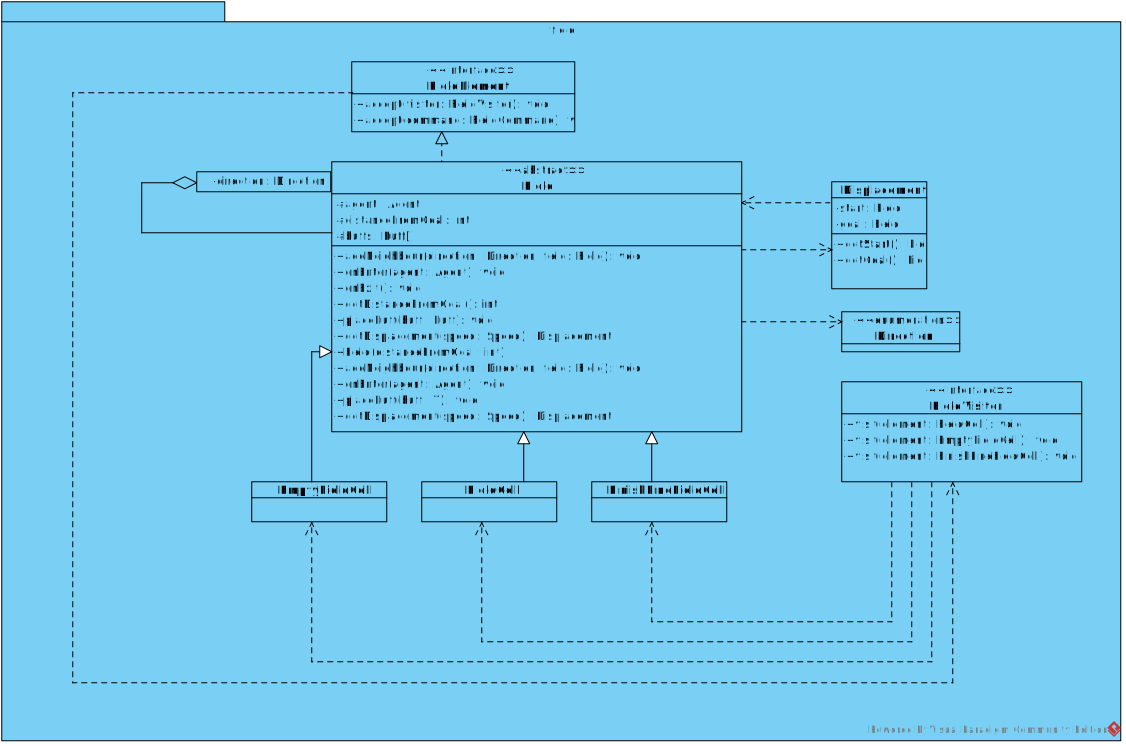
\includegraphics[width=\linewidth]{chapters/chapter03/ClassField.pdf}
\caption{Field package osztálydiagram}
\label{Field package osztálydiagram}
\end{center}
\end{figure}

\clearpage

\begin{figure}[h]
\begin{center}
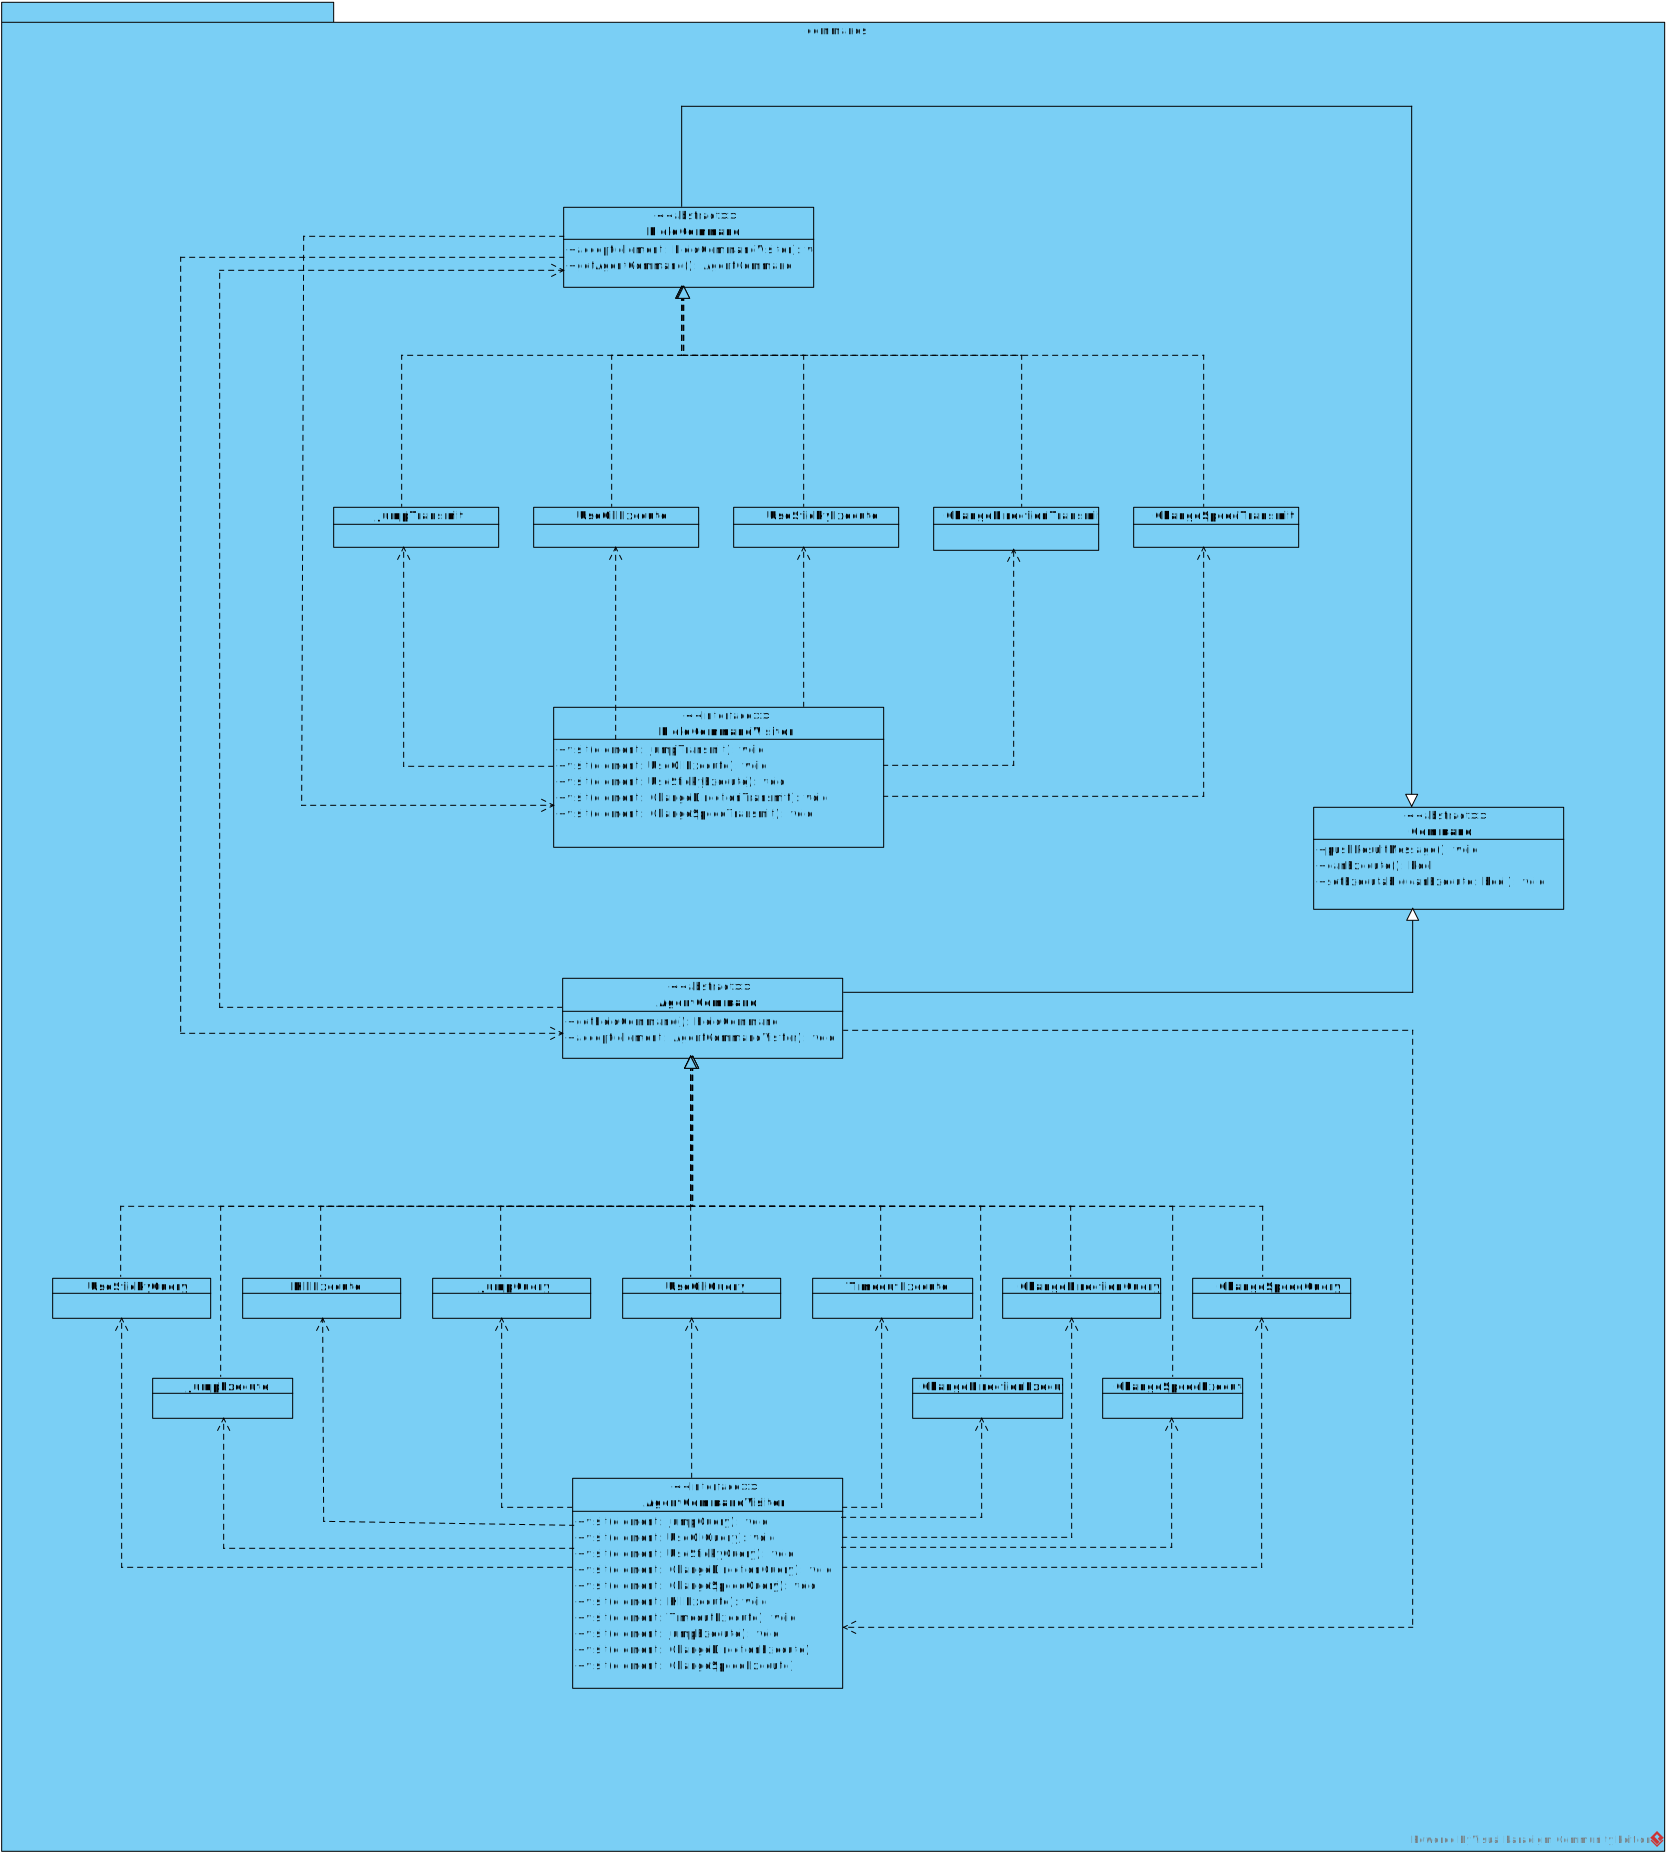
\includegraphics[width=\linewidth]{chapters/chapter03/ClassCommands.pdf}
\caption{Commands package osztálydiagram}
\label{Commands package osztálydiagram}
\end{center}
\end{figure}


\begin{figure}[h]
\begin{center}
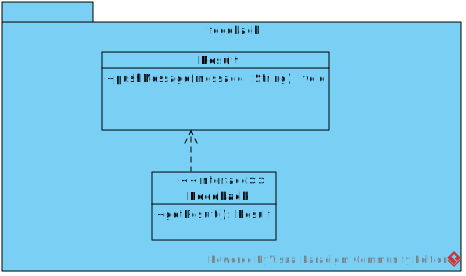
\includegraphics[width=\linewidth]{chapters/chapter03/ClassFeedback.pdf}
\caption{Feedback package osztálydiagram}
\label{Feedback package osztálydiagram}
\end{center}
\end{figure}


\begin{figure}[h]
\begin{center}
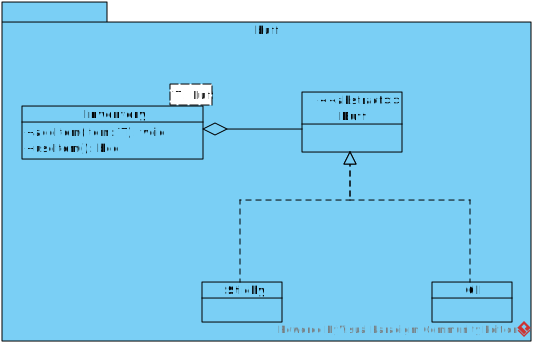
\includegraphics[width=\linewidth]{chapters/chapter03/ClassBuff.pdf}
\caption{Buff package osztálydiagram}
\label{Buff package osztálydiagram}
\end{center}
\end{figure}


\begin{figure}[h]
\begin{center}
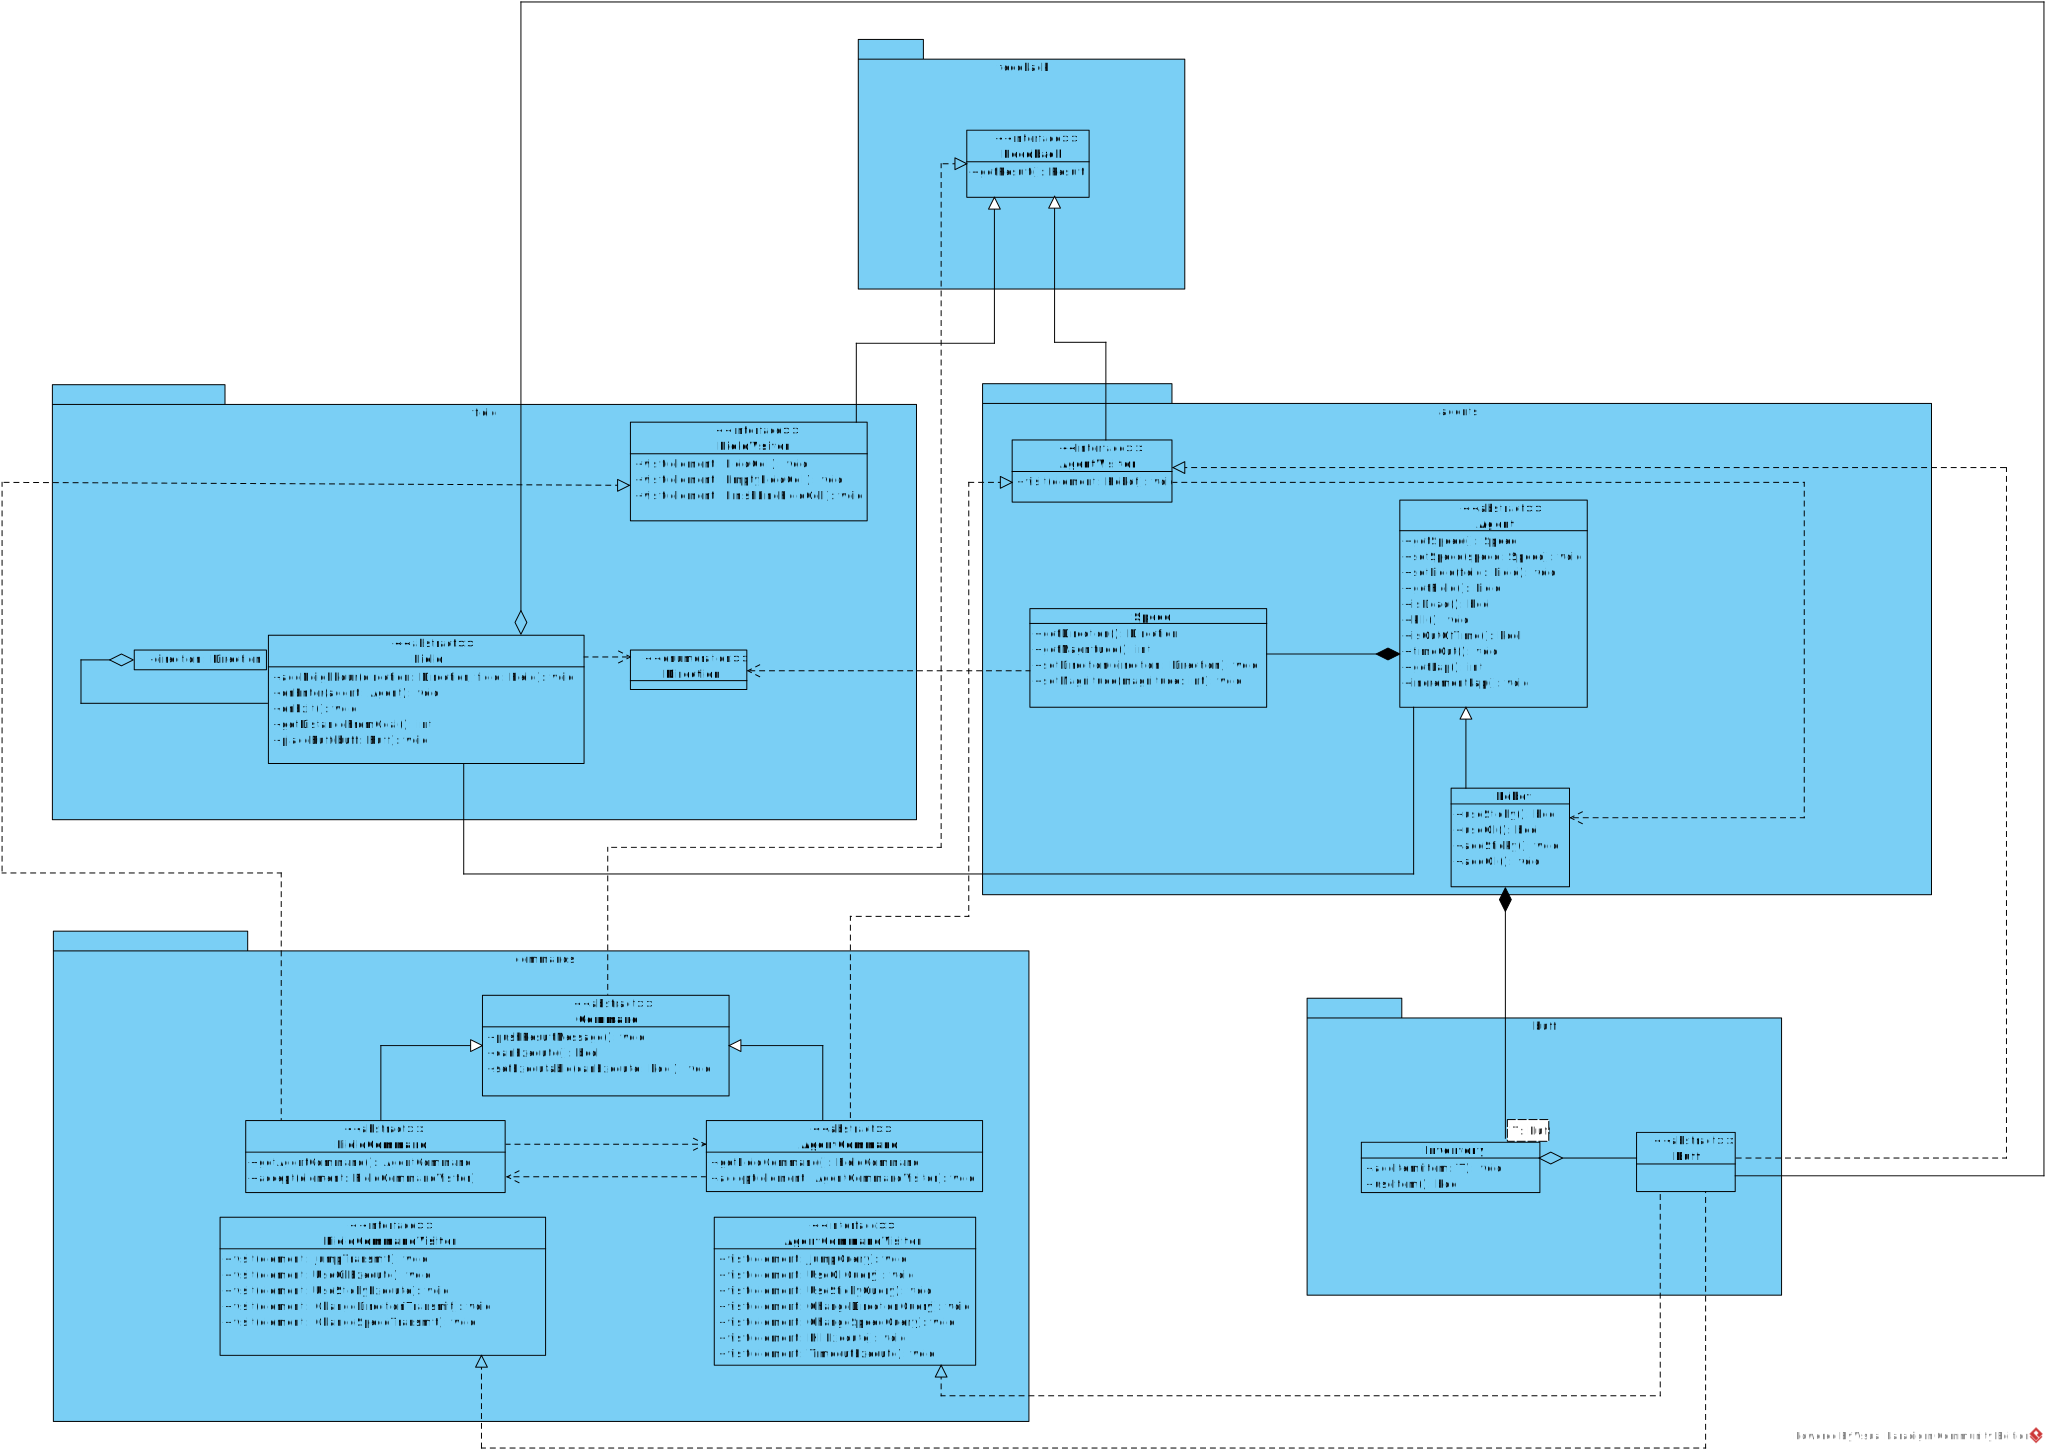
\includegraphics[width=\linewidth]{chapters/chapter03/ClassInterpackage.pdf}
\caption{Packagek közti függőségek osztálydiagramja}
\label{Packagek közti függőségek osztálydiagramja}
\end{center}
\end{figure}

\clearpage

\section{Szekvencia diagramok}

\begin{figure}[h]
	\begin{center}
		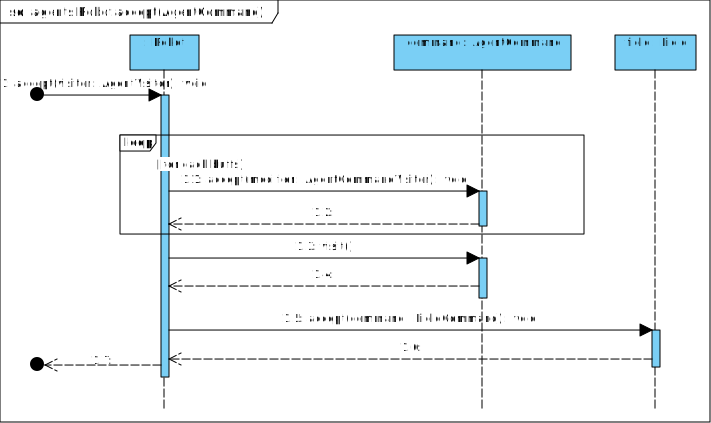
\includegraphics[width=\textwidth]{chapters/chapter03/agentsRobotacceptAgentCommand.pdf}
		\caption{Robot utasítást fogad}
		\label{fig:agents.Robot.accept}
	\end{center}
\end{figure}

\begin{figure}[h]
	\begin{center}
		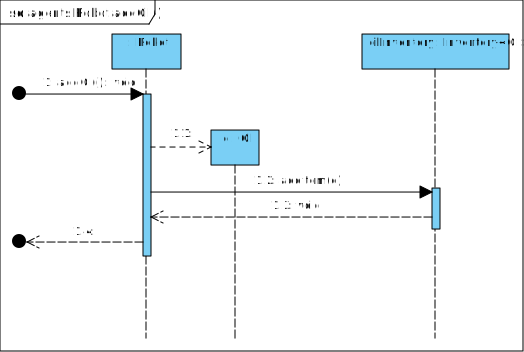
\includegraphics[width=\textwidth]{chapters/chapter03/agentsRobotaddOil.pdf}
		\caption{Robot felvesz a készletébe egy olajfoltot}
		\label{fig:agents.Robot.addOil}
	\end{center}
\end{figure}

\begin{figure}[h]
	\begin{center}
		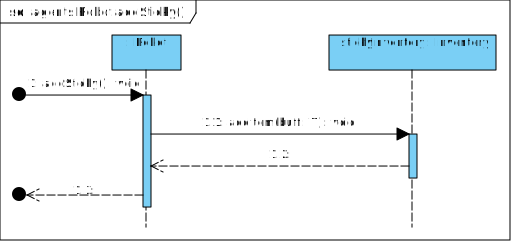
\includegraphics[width=\textwidth]{chapters/chapter03/agentsRobotaddSticky.pdf}
		\caption{Robot felvesz a készletébe egy ragacsfoltot}
		\label{fig:agents.Robot.addSticky}
	\end{center}
\end{figure}

\begin{figure}[h]
	\begin{center}
		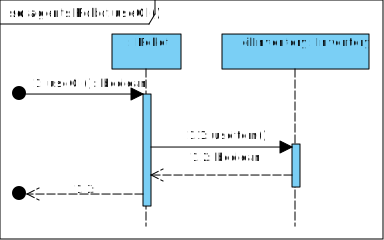
\includegraphics[width=\textwidth]{chapters/chapter03/agentsRobotuseOil.pdf}
		\caption{Robot felhasználja a készletében lévő olajfoltot ha van}
		\label{fig:agents.Robot.useOil}
	\end{center}
\end{figure}

\begin{figure}[h]
	\begin{center}
		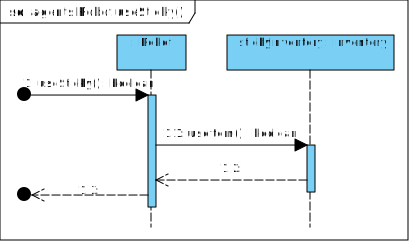
\includegraphics[width=\textwidth]{chapters/chapter03/agentsRobotuseSticky.pdf}
		\caption{Robot felhasználja a készletében lévő ragacsfoltot ha van}
		\label{fig:agents.Robot.useSticky}
	\end{center}
\end{figure}

\begin{figure}[h]
	\begin{center}
		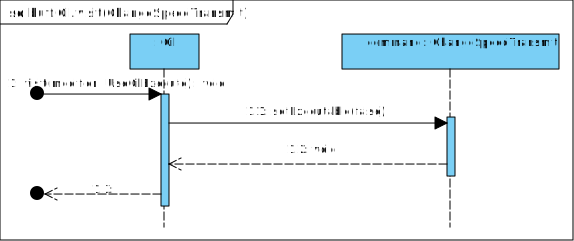
\includegraphics[width=\textwidth]{chapters/chapter03/buffOilvisitChangeSpeedTransmit.pdf}
		\caption{Olajfolt megakadályozza a sebesség nagyságának változtatását}
		\label{fig:buff.Oil.visit}
	\end{center}
\end{figure}

\begin{figure}[h]
	\begin{center}
		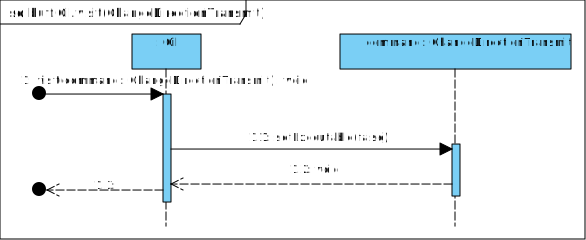
\includegraphics[width=\textwidth]{chapters/chapter03/buffOilvisitChangeDirectionTransmit.pdf}
		\caption{Olajfolt megakadályozza a sebesség irányának megváltoztatását}
		\label{fig:buff.Oil.visit2}
	\end{center}
\end{figure}

\begin{figure}[h]
	\begin{center}
		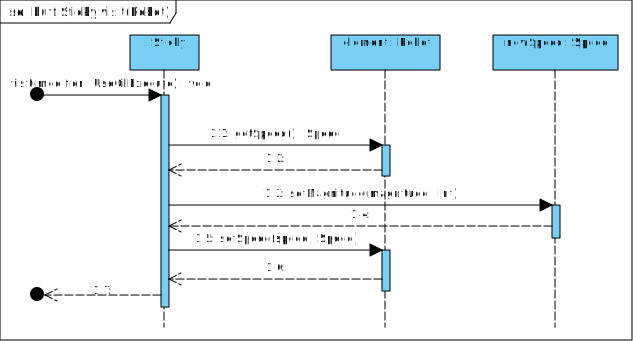
\includegraphics[width=\textwidth]{chapters/chapter03/buffStickyvisitRobot.pdf}
		\caption{Olajfolt megakadályozza a sebességváltoztatást}
		\label{fig:buff.Sticky.visit}
	\end{center}
\end{figure}

\begin{figure}[h]
	\begin{center}
		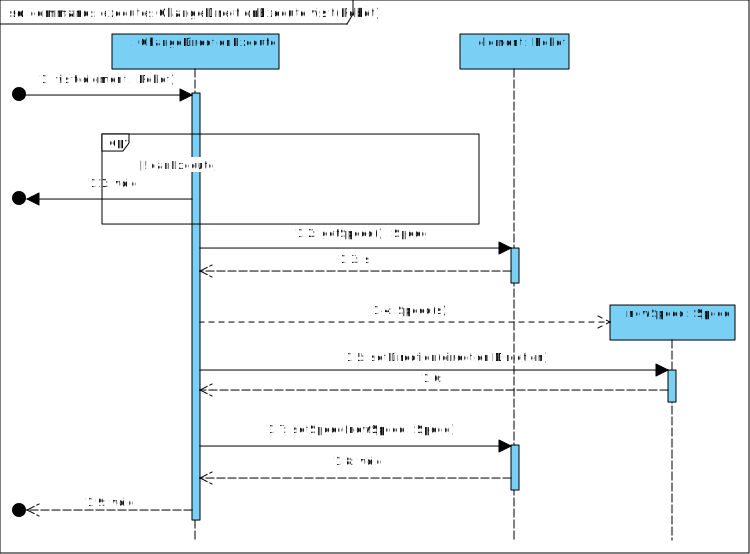
\includegraphics[width=\textwidth]{chapters/chapter03/commandsexecutesChangeDirectionExecutevisitRobot.pdf}
		\caption{Robot irányváltoztatásának végrehajtása}
		\label{fig:command.executes.ChangeDirectionExecute.visit}
	\end{center}
\end{figure}

\begin{figure}[h]
	\begin{center}
		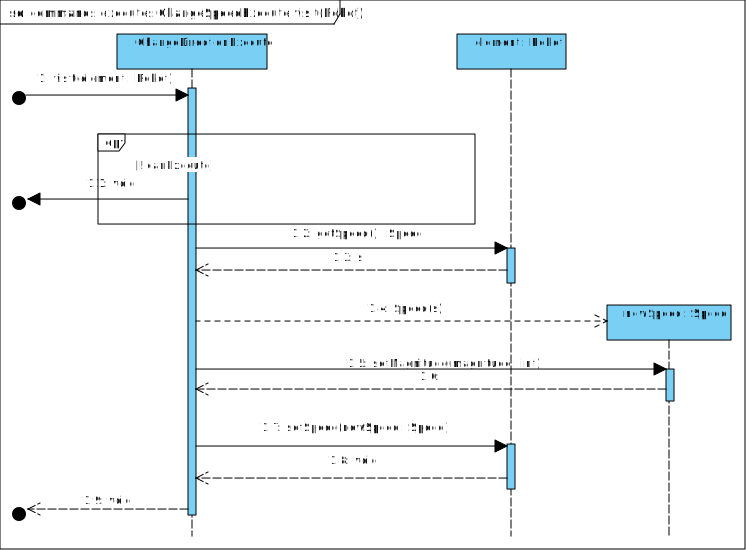
\includegraphics[width=\textwidth]{chapters/chapter03/commandsexecutesChangeSpeedExecutevisitRobot.pdf}
		\caption{Robot sebességnagyságának megváltoztatása}
		\label{fig:command.executes.ChangeSpeedExecute.visit}
	\end{center}
\end{figure}

\begin{figure}[h]
	\begin{center}
		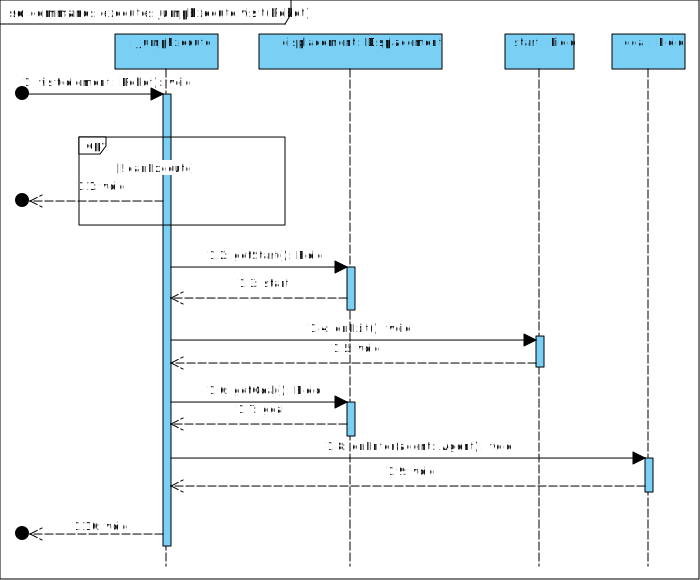
\includegraphics[width=\textwidth]{chapters/chapter03/commandsexecutesJumpExecutevisitRobot.pdf}
		\caption{Robot ugrásának végrehajtása}
		\label{fig:command.executes.JumpExecute.visit}
	\end{center}
\end{figure}

\begin{figure}[h]
	\begin{center}
		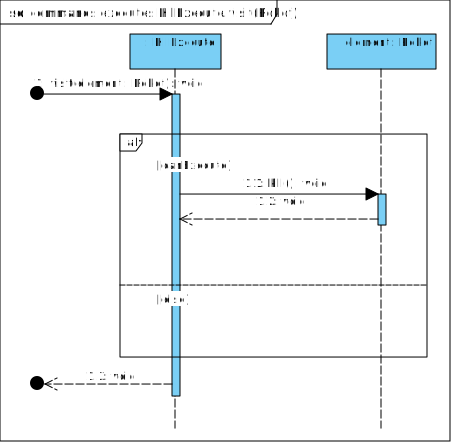
\includegraphics[width=\textwidth]{chapters/chapter03/commandsexecutesKillExecutevisitRobot.pdf}
		\caption{Robot megölésének végrehajtása}
		\label{fig:command.executes.KillExecute.visit}
	\end{center}
\end{figure}

\begin{figure}[h]
	\begin{center}
		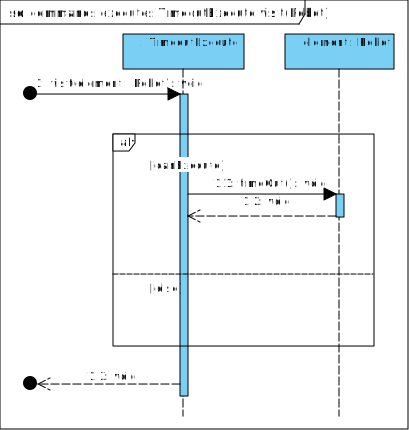
\includegraphics[width=\textwidth]{chapters/chapter03/commandsexecutesTimeoutExecutevisitRobot.pdf}
		\caption{Robot idő lejártának végrehajtása}
		\label{fig:command.executes.TimeoutExecute.visit}
	\end{center}
\end{figure}

\begin{figure}[h]
	\begin{center}
		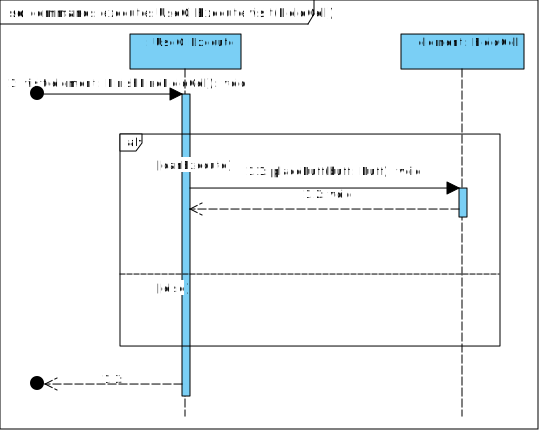
\includegraphics[width=\textwidth]{chapters/chapter03/commandsexecutesUseOilExecutevisitFieldCell.pdf}
		\caption{Robot lehelyezi az Olaj foltot a mezőre}
		\label{fig:command.executes.UseOilExecute.visit}
	\end{center}
\end{figure}

\begin{figure}[h]
	\begin{center}
		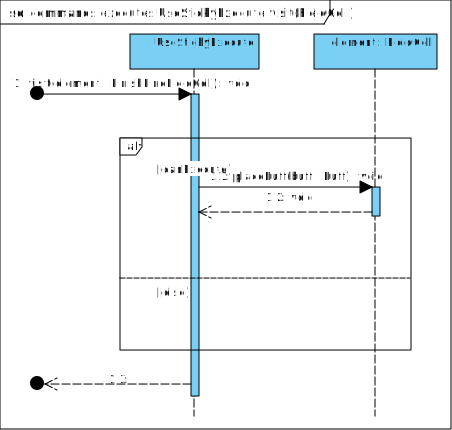
\includegraphics[width=\textwidth]{chapters/chapter03/commandsexecutesUseStickyExecutevisitFieldCell.pdf}
		\caption{Robot lehelyezi a Ragacs foltot a mezőre}
		\label{fig:command.executes.UseStickyExecute.visit}
	\end{center}
\end{figure}

\clearpage

\begin{figure}[h]
	\begin{center}
		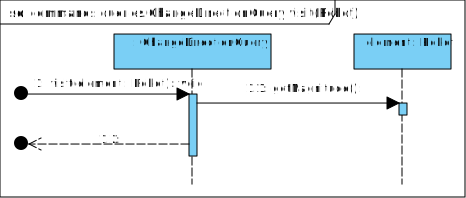
\includegraphics[width=\textwidth]{chapters/chapter03/commandsqueriesChangeDirectionQueryvisitRobot.pdf}
		\caption{Robot irányváltásra való felkérése}
		\label{fig:command.executes.ChangeDirectionQuery.visit}
	\end{center}
\end{figure}

\begin{figure}[h]
	\begin{center}
		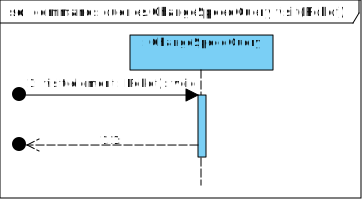
\includegraphics[width=\textwidth]{chapters/chapter03/commandsqueriesChangeSpeedQueryvisitRobot.pdf}
		\caption{Robot sebesség nagyságának megváltoztatására való felkérése}
		\label{fig:command.executes.ChangeSpeedQuery.visit}
	\end{center}
\end{figure}

\begin{figure}[h]
	\begin{center}
		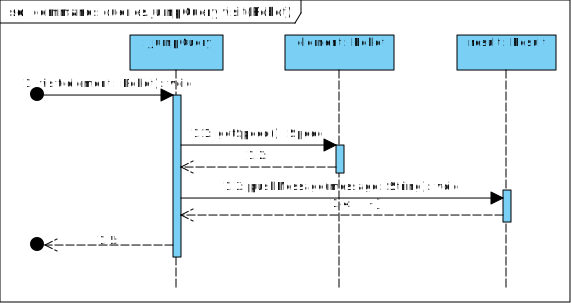
\includegraphics[width=\textwidth]{chapters/chapter03/commandsqueriesJumpQueryvisitRobot.pdf}
		\caption{Robot ugrásra azaz helyzetmódosításra való felkérése}
		\label{fig:command.executes.JumpQuery.visit}
	\end{center}
\end{figure}

\begin{figure}[h]
	\begin{center}
		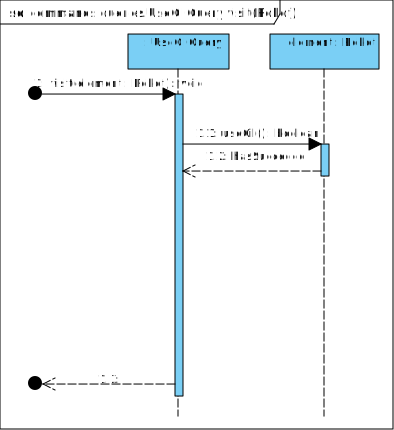
\includegraphics[width=\textwidth]{chapters/chapter03/commandsqueriesUseOilQueryvisitRobot.pdf}
		\caption{Robotot Olaj lehelyezésére való felkérése}
		\label{fig:command.executes.UseOilQuery.visit}
	\end{center}
\end{figure}

\begin{figure}[h]
	\begin{center}
		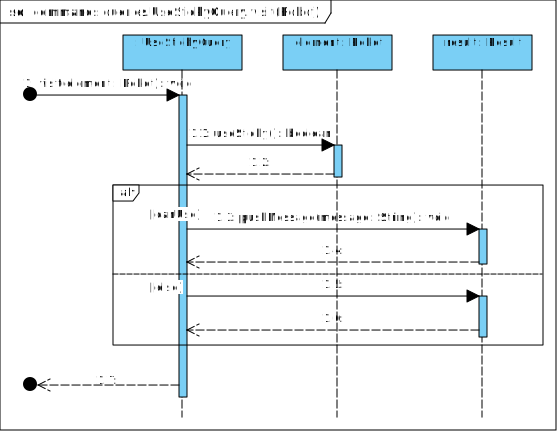
\includegraphics[width=\textwidth]{chapters/chapter03/commandsqueriesUseStickyQueryvisitRobot.pdf}
		\caption{Robotot Ragacs lehelyezésére való felkérése}
		\label{fig:command.executes.UseStickyQuery.visit}
	\end{center}
\end{figure}

\begin{figure}[h]
	\begin{center}
		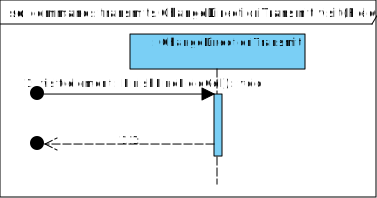
\includegraphics[width=\textwidth]{chapters/chapter03/commandstransmitsChangeDirectionTransmitvisitFieldCell.pdf}
		\caption{Irányváltásra vonatkozó kérés átvitele}
		\label{fig:command.executes.ChangeDirectionTransmit.visit}
	\end{center}
\end{figure}

\begin{figure}[h]
	\begin{center}
		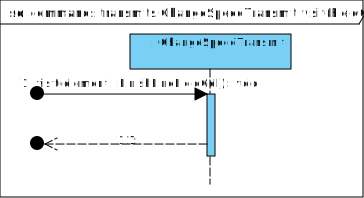
\includegraphics[width=\textwidth]{chapters/chapter03/commandstransmitsChangeSpeedTransmitvisitFieldCell.pdf}
		\caption{Szebességnagyság változtatásra vonatkozó kérés átvitele}
		\label{fig:command.executes.ChangeSpeedTransmit.visit}
	\end{center}
\end{figure}

\begin{figure}[h]
	\begin{center}
		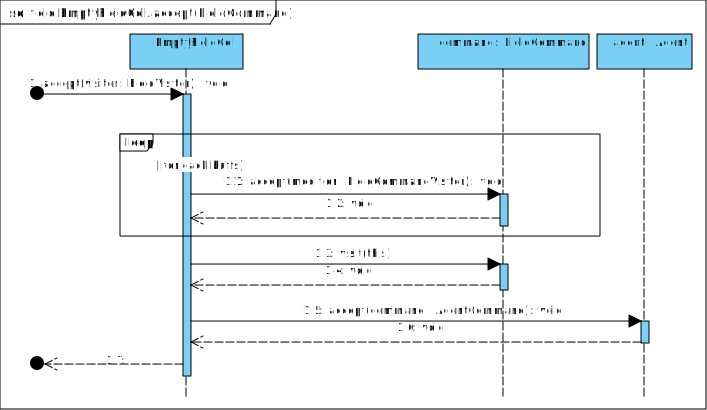
\includegraphics[width=\textwidth]{chapters/chapter03/fieldEmptyFieldCellacceptFieldCommand.pdf}
		\caption{Üres pályamező utasításfeldolgozása}
		\label{fig:field.EmptyFieldCell.accept}
	\end{center}
\end{figure}

\begin{figure}[h]
	\begin{center}
		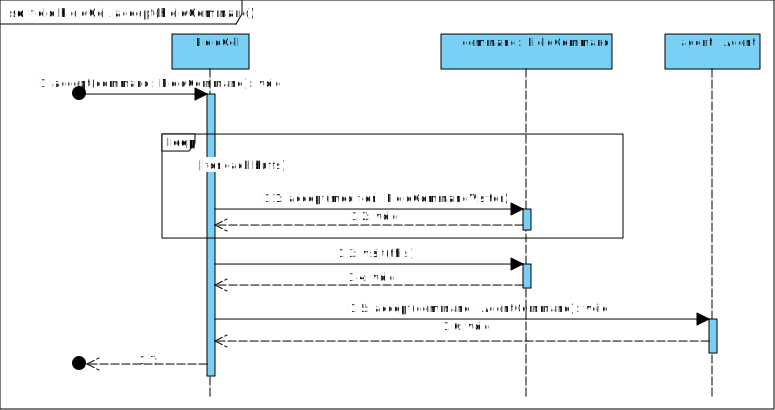
\includegraphics[width=\textwidth]{chapters/chapter03/fieldFieldCellacceptFieldCommand.pdf}
		\caption{Pályamező utasításfeldolgozása}
		\label{fig:field.FieldCell.accept}
	\end{center}
\end{figure}

\begin{figure}[h]
	\begin{center}
		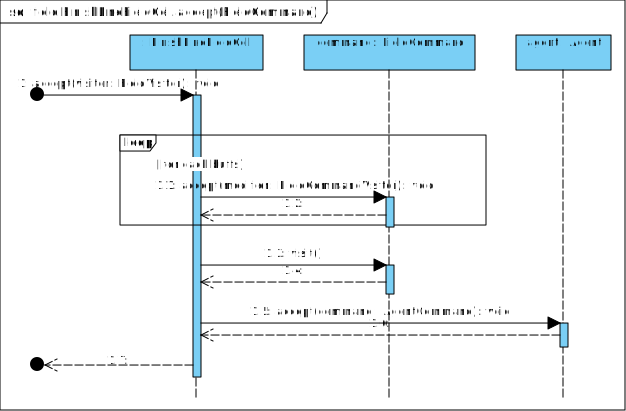
\includegraphics[width=\textwidth]{chapters/chapter03/fieldFinishLineFieldCellacceptFieldCommand.pdf}
		\caption{Start/célvonal pályamező utasításfeldolgozása}
		\label{fig:field.FinishLineFieldCell.accept}
	\end{center}
\end{figure}

\clearpage

\section{State-chartok}
\comment{Csak azokhoz az osztályokhoz, ahol van értelme. Egyetlen állapotból álló state-chartok ne szerepeljenek. A játék működését bemutató state-chart-ot készíteni tilos.}

\begin{figure}[h]
\begin{center}
%\includegraphics[width=17cm]{chapters/chapter03/example.pdf}
\caption{x}
\label{fig:example3}
\end{center}
\end{figure}

